\documentclass[9pt]{beamer}
\usetheme{Madrid}
\usepackage{mathtools}
\usepackage{bm}
\usepackage{esvect}
\usepackage{amsmath}
\usepackage{physics}
\usepackage{empheq}
\usepackage[many]{tcolorbox}

%$\vv{\bm{L}}

\title{Where is everybody?}
 
\subtitle{A possible solution to the Fermi Paradox}
 
\author{J.J. G\'omez Cadenas}
 
\institute{Donostia International Physics Center (DIPC)} % (optional)
 
\date[October 6th, 2018] % (optional)
{PHYSIS, SAN SEBASTIAN: 2-6 OCTOBER 2018}
 
\logo{\includegraphics[height=0.5cm]{dipc.png}
\includegraphics[height=0.5cm]{IB.png}}


\tcbset{highlight math style={enhanced,
  colframe=red!60!black,colback=yellow!50!white,arc=4pt,boxrule=1pt,
  }}

\newtcbox{\mybox}[1][]{nobeforeafter,math upper,tcbox raise base,
  enhanced,frame hidden,boxrule=0pt,interior style={top color=green!10!white,
  bottom color=green!10!white,middle color=green!50!yellow},
  fuzzy halo=1pt with green,drop large lifted shadow,#1}
\begin{document}

\frame{\titlepage}

%%%%%%%%%%%%%%

\begin{frame}
\frametitle{A reasonable theory}

\begin{columns}
\column{0.35\textwidth}
\includegraphics[scale=0.3]{aliens}
New Yorker cartoon by Alan Dunn in the New Yorker


 \column{0.5\textwidth}
%\begin{block}{}
In the Spring of 1950 the New York newspapers reported simultaneously the disappearance of public trash cans and numerous flying saucer observations. 
\vspace{0.5cm}

Fermi was at Los Alamos in the summer of 1950. One day, he was chatting to Edward Teller and Herbert York and Emil Konopinski told them of the Dunn cartoon. Fermi remarked wryly that Dunn's was a reasonable theory because it accounted for two distinct phenomena: the disappearance of trash cans and the reports of flying saucers. 
%\end{block}
\end{columns}
\end{frame}

%%%%%%%%%%%%%%%%
\begin{frame}
\frametitle{Where is everybody?}

\begin{columns}
\column{0.40\textwidth}
\includegraphics[scale=0.25]{aliensfermi.jpeg}

 \column{0.5\textwidth}
\begin{itemize}

\item During lunch Fermi asked suddenly: ``Where is everybody?'' His lunch partners immediately understood that he was talking about aliens. York recalls that Fermi made a series of rapid calculations and concluded that we should have been visited long ago and many times over.

\item Apparently Fermi didn’t saw the outcome of his calculation as a paradox. He also didn't doubt that extraterrestrial civilizations might exist, but supposed that interstellar travel wasn’t feasible or that alien had simply never found Earth in the vastness of the galaxy.    
\end{columns}
\end{frame}

%%%%%%%%%%%%%%%
\begin{frame}
\frametitle{The Drake equation}

\begin{columns}
\column{0.40\textwidth}
\includegraphics[scale=0.25]{drake}

 \column{0.5\textwidth}
\begin{itemize}

\item Represent the number of communicating Extraterrestrial Civilizations (ETCs) in the Galaxy by the symbol $N$. To estimate $N$ we multiply the following factors: the yearly rate $R$ at which stars form in the Galaxy; the fraction $f_p$ of stars that possess planets; the fraction $n_e$ of planets with environments suitable for life. The fraction $f_l$ of suitable planets on which life actually develops; the fraction of these planets on which life develops intelligence $f$; and the fraction $f_c$ of intelligent life-forms that develop a culture capable of interstellar communication. Finally, we need to know the time $L$, in years, that such a culture will devote to communication. Multiplying all these factors together results in the famous Drake's equation.

\item The Drake equation is a means of estimating the number of communicative ETCs in the Galaxy. Drake developed the equation so that it could form the agenda for the first ever SETI meeting (held at nrao Green Bank, WV, in 1961). The commemorative plaque is on the same wall that held the blackboard where the equation was first written.   
\end{columns}
\end{frame}
%%%%%%%%%%%%%%%%%

\begin{frame}
\frametitle{The Hart-Tipler argument}

\begin{columns}
\column{0.40\textwidth}
\includegraphics[scale=0.25]{spaceships}

Hart, Michael H. “Explanation for the Absence of Extraterrestrials on Earth.” Quarterly Journal of the Royal Astronomical Society, Vol. 16, 1975, pp.128–135.

“an extensive search for radio messages from other civilizations is probably a waste of time and money”


 \column{0.5\textwidth}
\begin{itemize}

\item In his 1975 paper, astronomer M. Hart speculated how long it would take hypothetical alien civilizations to colonize the Miky Way. He assumed that space-faring alien civilizations could proliferate with a colonization wavefront speed of 10 percent the speed of light (equal to the speed that colonization ships could spread throughout the galaxy). Given that the Milky Way is about 100 Myr across, colonization would take  about 1Myr, a tiny span of time compared with the age of the galaxy. 

\item Hart used this reasoning to argue for the nonexistence of advanced extraterrestrials in the Milky Way, since humans (latecomers in the history of the galaxy) have not found signs of their probes or colonization ships (nor any meaningful signal emitted by putative ``galactic centers''. Hart equated lack of observation to non-existence.  
\end{columns}
\end{frame}


%%%%%%%%%%%%%

\begin{frame}
\frametitle{The Neuman-Sagan  model}

\begin{columns}
\column{0.40\textwidth}
\includegraphics[scale=0.25]{spaceships}

Icarus, Volume 46, Issue 3, June 1981, Pages 293-327.

 \column{0.5\textwidth}
\begin{itemize}

\item In his 1975 paper, astronomer M. Hart speculated how long it would take hypothetical alien civilizations to colonize the Miky Way. He assumed that space-faring alien civilizations could proliferate with a colonization wavefront speed of 10 percent the speed of light (equal to the speed that colonization ships could spread throughout the galaxy). Given that the Milky Way is about 100 Myr across, colonization would take  about 1Myr, a tiny span of time compared with the age of the galaxy. 

\item Hart used this reasoning to argue for the nonexistence of advanced extraterrestrials in the Milky Way, since humans (latecomers in the history of the galaxy) have not found signs of their probes or colonization ships (nor any meaningful signal emitted by putative ``galactic centers''. Hart equated lack of observation to non-existence.  
\end{columns}
\end{frame}


%%%%%%%%%

%\begin{frame}
%%\frametitle{FP revisited}
%\begin{block}{}
%\center{\Huge FP Revisited}
%\end{block}
%\end{frame}

\begin{frame}
\frametitle{Formulations of the Fermi Paradox}
\begin{itemize}
\item {\bf ProtoFP}: The absence of extraterrestrials on Earth is incompatible with the multiplicity of extraterrestrial civilisations and our conventional assumptions about their capacities. 
\item {\bf WeakFP}: The absence of extraterrestrials or their artefacts on Earth and in the Solar System is incompatible with the multiplicity of extraterrestrial civilisations and our conventional assumptions about their capacities. ProtoFP and WearkFP are {\em weak} formulations of the FP, since, even in a Galaxy teeming with advanced civilisations, there are many ways to explain non-direct observations {\em on Earth or the solar system}.
\item {\bf StrongFP}: The lack of any intentional activities or manifestations or traces of extraterrestrial civilisations in our past light cone is incompatible with the multiplicity of extraterrestrial civilisations and our conventional assumptions about their capacities. This is much hard to explain, since it involves a much larger volume (thus many more potential civilisations) and tries to detect any signal arising from them. As an example, our primitive Earth civilisation has been signalling its presence of the last two hundred years or so. 
\end{itemize}

\end{frame}

%\begin{frame}
%\frametitle{More paradoxical than ever}
%
%\begin{columns}
%\column{0.35\textwidth}
%\includegraphics[scale=0.03]{earthlike.jpeg}
%
%The number of Sun-like stars that could have an Earth-like planet in the habitable zone may be as high as  22\%. 
%
%%(https://www.pnas.org/doi/full/10.1073/pnas.1319909110)
%
%
% \column{0.5\textwidth}
%%\begin{block}{}
%
%A number of recent discoveries make the problem objectively more disturbing than ever.
%
%\vspace{0.5cm}
%
%For example: in 1950 one could argue that planetary solar systems were rare (or even unique), or that ``Goldilocks'' conditions happened exceptionally or  that Earth is in the extreme early tail of the planet-age distribution, being among the oldest, if not the oldest habitable planet in the Milky Way. Those hypothesis, not unreasonable at the time would have ``solved'' the paradox, leading to Earth being the first civilisation in the Galaxy. 
%\end{columns}
%\end{frame}
%
%\begin{frame}
%\frametitle{Recent scientific advances suggest we are not singular}
%\begin{itemize}
%\item Confirmation of the rapid origination of life
%on early Earth (Mojzsis et al. 1996) offers a strong probabilistic
%support to the idea of many planets in the
%Milky Way inhabited by at least the simplest
%lifeforms (Lineweaver and Davis 2002).
%\item Discovery of extremophiles and the general resistance of simple lifeforms to much more severe environmental stresses than it had been
%thought possible earlier (Cavicchioli 2002) suggests that the number and
%variety of cosmic habitats for life are probably
%much larger than conventionally imagined.
%\item Improved understanding in molecular biology and biochemistry leading to heightened
%confidence in the theories of naturalistic origin
%of life or {\em abiogenesis} (Lahav et al. 2001, Ehrenfreund et al. 2002, Bada 2004). 
%\item Improved understanding of the origin of intelligence and technological civilization
%({\em noogenesis}) also supports naturalistic origin (e.g. Chernavskii 2000).
%\end{itemize}
%
%\begin{block}{}
%In short, recent scientific advances suggest that life and (to a lesser degree) intelligence should be common in the Universe. 
%\end{block}
%\end{frame}
%
%\begin{frame}
%\frametitle{Technological advances suggest that Galaxy colonisation is possible}
%\begin{itemize}
%\item Exponential growth of the technological civilization on Earth (e.g., technological waves of which IAG is the last, see Suleiman 2023) suggests that civilisations
% experience exponential technological grow. 
%\item An outstanding question is whether energy will limit technological development on Earth. The optimistic view is that it will not. Technological civilisations can harness eventually nuclear fusion as well as (all) the energy provided by their star. 
%\item Interstellar travel appears more feasible in both the classical sense
%(e.g. Andrews 2003), and in the more efficient
%form of sending interstellar probes.
%%\item Theoretical grounding for various astroengi-
%%neering/macroengineering projects (Badescu
%%1995, Badescu and Cathcart 2000, 2006, Ko-
%%rycansky et al. 2001, McInnes 2002) potentially detectable over interstellar distances.
%%Especially important in this respect is the
%%possible combination of astroengineering and
%%computation projects of advanced civiliza-
%%tions, like those envisaged by Sandberg (1999).
%\item We have observed many galaxies, and not a single civilization of Kardashev's Type III has been
%found, in spite of the huge volume of space
%surveyed (Annis 1999b).
%\end{itemize}
%
%\begin{block}{}
%StrongFP is a more paradoxical than ever.  
%\end{block}
%\end{frame}

\begin{frame}
\frametitle{Kardashev Classification}

\includegraphics[scale=0.15]{kardashev.png}

The Kardashev scale (1964) ranks the technological capabilities of a civilization based on its ability to manipulate and exploit energy. 
\begin{itemize}
\item {\bf Type 0} uses energy sources like coal, oil, and natural gas.
\item {\bf Type I} has complete control over the energy of its host planet.
\item {\bf Type II} can harness the power of its sun and control the entire solar system.
\item {\bf Type III} spans the entire galaxy, colonizing and controlling numerous systems. 
\end{itemize}

Humanity is considered a type 0 civilization (0.72 according to Carl Sagan). It is estimated that we will reach type I in 100–200 years, type II in $\sim$ 10 kyrs, and type III in $10^5--10^6$ to kyrs.

\end{frame}

\begin{frame}
\frametitle{Fermi-Hart timescale}

\begin{columns}
\column{0.5\textwidth}
\includegraphics[scale=0.5]{colonisation.png} 

 \column{0.4\textwidth}
Fermi’s paradox in a model with slow von Neumann probes, giving a typically low Fermi-Hart timescale for the colonization of the Milky Way. The relevant timescales are also shown.

$t_{FH} \sim 10^6-10^8$ yr
\end{columns}
\end{frame}
\begin{frame}
\frametitle{The Galaxy-Solar system timescale}

\includegraphics[scale=0.45]{M00s9.png}


The formation of Earth-like planets started likely more than 9 Gyr ago. The median age of planes in the galaxy is $t_M =6.4 \pm 0.9$ Gyr, while the solar system (and Earth) have an age $t_E =4.5681 \pm 0.004$ Gyr. This means that planet formation in the galaxy reached its peak  $t_M - t_E = 1.9 \pm 0.9$ Gyr before our planet completed its original accretion. Also, consider that the older planes formed $\sim$ 4 Gyr before Earth.  

\end{frame}

\begin{frame}
\frametitle{The FP reformulated}

\begin{block}{}

$$ t_{FH} <<< t_M - t_E$$

\end{block}

\vspace{0.5cm}
\begin{itemize}
\item
Most of the habitable sites in the Milky Way (and most likely elsewhere) are billions of years older than Earth, giving ample time for KTIII civilisations to form. Thus, the Galaxy should be already colonized and/or, evidence for KTIII civilisations in other galaxies should be observable. 
%
%\vspace{0.5cm}
\item
Even more generally, we need not consider the direct physical contact between an extraterrestrial civilization and Earth or the Solar System. It is sufficient to consider a weaker requirement: namely that no extraterrestrial civilizations are detectable by any means from Earth at present. In particle physics parlance we could ask why the ``contact cross-section'' in the Milky Way at present is so small in comparison to naive expectations.
\end{itemize}
%{\em provided that we accept the straightforward Copernican assumption}.
%\end{columns}
%\end{frame}
\end{frame}

\begin{frame}
\frametitle{The Philosophy department's nightmare.}

{\em Hi guys, we are physicist and we are here to help!}
\vspace{0.5cm}

Disclaimers: 

\begin{itemize}
\item In this talk I am going to use profusely terms  such as``intuitive'', ``accepted'', ``common sense'', ``practical'', or ``effective''.  If you feel that I am trying to avoid rigorous definitions, talk to my lawyer.  
\item Since I am not providing a rigorous definition of ``intelligence''  (or, God forbids, ``conscience''), then I don't need to be precise when referring to ``extraterrestrial intelligence''. Extraterrestrial intelligent beings are taken as entities which are able to communicate with. 
\item I will stick to a few philosophical concepts as ``desirable guides'' to understand FP. Specifically, I will invoke Realism, Naturalism, Copernicanism, Gradualism (this one tongue-in-cheek) and Hardness as guidelines to  ``grade'' potential explanations of the FP. In my definitions of the above ``ism's'' I will also be ``intuitive'', and my ``grading'' may be totally biased. Again, my lawyer will be happy to discuss any pertinent legal issues with those of you who rather chase me out of the room.  
\end{itemize}

\end{frame}

%\begin{frame}
%\frametitle{Key concepts related with Fermi Paradox}
%
%\begin{columns}
%\column{0.35\textwidth}
%\includegraphics[scale=0.06]{impossible.jpeg}
%
%Fermi Paradox may sits well into a famous class of mathematical problems popularised by Martin Gardner and often known as "impossible puzzles",
%
%
% \column{0.5\textwidth}
%%\begin{block}{}
%Scientific and technological: Intelligence, civilisation, technology, evolution, interstellar travel, detectability. Philosophical:  Realism, Copernican assumption, naturalism,  to name a few. 
%
%\vspace{0.5cm}
%
%The Paradox sits well into a famous class of mathematical problems popularised by Martin Gardner and often known as "impossible puzzles", where players have insufficient information to produce a solution, but gain additional knowledge from the fact that the other players cannot solve it either.
%
%%\end{block}
%\end{columns}
%\end{frame}



%\begin{frame}
%\frametitle{Detectability \& synchronisation}
%
%\begin{itemize}
%\item {\bf Detectability} of an intelligent species is a metric quantifying the difficulty to detect the presence of such a species from interstellar distances. The {\em soft} detectability condition would apply to detectability within the Galaxy, thus a range from less than a parsec to several thousand parsecs. The {\em hard} condition would extend detectability to species in the past light cone (e.g., the set of accesible galaxies from our view point). 
%\item {\bf Synchronisation}  implies that other intelligent species are contemporary to us, a concept way more restrictive than detectability. 
%\end{itemize}

%\end{frame}

\begin{frame}
\frametitle{Philosophical handles: Realism}

\begin{itemize}
\item {\bf Scientific, ``naive'' or ``common sense'' realism}.  Working philosophy of most of science (as well as everyday life), implying that there is a material world out there, composed of objects that occupy space, have a duration in time, and have properties such as size, mass, shape, texture, smell, taste, and colour. These properties are usually perceived correctly and obey the laws of physics. 
\item {\bf Realism applied to FP} states that there are no traces of extraterrestrial intelligent presence (ETI) detected either directly or indirectly.

\item {\bf Realism is a methodological assumption} used in scientific research. Neither me, nor my lawyer will consider as valid solutions of FP that violate the Realism requirement (e.g., UFO = ETI theories).  
\end{itemize}

\end{frame}

\begin{frame}
\frametitle{Philosophical handles: Naturalism}

{\em Monsiuer, Je n'avais pas besoin the cette hypotehèse (Laplace to the First Consul of French Republic). }

\vspace{0.5 cm}
\begin{itemize}
\item A prohibition against invoking supernatural agents or events in scientific explanations.
\item Naturalism (at least on its soft version, which is good enough for this discussion) does not make hypothesis concerning the existence of supernatural agents, it just states that our explanatory mechanism should not invoke them either explicitly or implicitly.
\item Indeed, supernaturalism could solve easily the FP by postulating a unique divine creation in the Universe, as in Western monotheistic religions (although one could need to explain why the waste of resources, e.g, $10^{22}$ stars for a single inhabited planet). 
\end{itemize}
\end{frame}


\begin{frame}
\frametitle{Naturalism and Abiogenesis}

\begin{itemize}
\item A necessary (naturalist) ingredient in any scientific account of life is the so-called {\bf continuity thesis}, that is the assumption that there is no unbridgeable gap between inorganic matter and living systems.
\item On the other hand, the question of how probable is the emergence of life has not been fully quantified. While the prevalent scientific view is that given the
 right physical conditions the emergence of life is highly probable, this is not a demonstrated fact, since we do not have yet a full description of the mechanisms that led to life from inorganic matter, nor have we been able to ``replicate'' life in the lab. 
\item An scenario in which the emergence of life turned out to be extremely improbable, could act as an ``early filter'' that would solve the FP, providing an explanation which would be ``de facto'' identical to the supernatural ``divine creation'' hypothesis mentioned above, while still respecting naturalism (extremely improbable does not mean impossible).  
\end{itemize}
\end{frame}

\begin{frame}
\frametitle{Naturalism and Noogenesis}

\begin{itemize}
\item The continuity thesis should also apply to the emergence of ``intelligence'' and ``conscience''. The situation here is more complex, since it is difficult to define what intelligence (or conscience) means.
\item On the other hand one could argue that intelligence (and conscience) are common phenomena on Earth. Examples of intelligent species include dolphins, whales and the great apes. We know of at least an intelligent Homo species (Neanderthals) not equivalent to Sapiens. Thus one could expect that the emergence of intelligence, once complex life evolves is highly probable.  
\item In 2023 is specially relevant to consider also post-biological intelligence, e.g, the emergence of (imminent?)  artificial intelligence.  Notice that many of the technical difficulties associated with interstellar travel (and thus to the expansion of advanced civilizations) only apply to biological, not post-biological (``machines'') beings, which could be the predominant form of intelligence in the Galaxy. 
\end{itemize}
\end{frame}

\begin{frame}
\frametitle{Philosophical handles: Copernicanism}
\begin{itemize}
\item {\bf Also called Principle of Typicality}. There is nothing special about Earth, the Solar System, or our Galaxy within large sets of similar objects throughout the universe (Sagan, Drake and others). In a somewhat broader sense, it indicates that there is nothing special about us as observers: our temporal or spatial location, or our location in other abstract spaces of physical parameters, chemical parameters, biological parameters, and so on, are typical or close to typical. 
\item Notice that, unlike Realism and Naturalism, Copernicanism is not a scientific must, although it has been a cornerstone of the scientific revolution and the ``great demotions'' that took Earth (and man) out of the center of the Universe. And yet, nothing prevents our planet, {\em a priory} from being an outlier in one or more aspects. As we will see soon, a full family of proposed solutions to the FP, grouped under the label of ``Rare Earth Hypothesis'' argue precisely so. 
\end{itemize}

\end{frame}

\begin{frame}
\frametitle{Philosophical handles: Non-exclusivity}
\begin{itemize}
\item {\bf Also called Principle of Hardness}.  Favours those hypotheses which involve a smaller number of local causes. 
\item For example, the FP  is not resolved by postulating that the Galaxy contained only one  single old civilisation (apart of us), which self-destructed itself in a nuclear holocaust (why just one?). Instead we would need to postulate that all civilizations self-destruct soon after developing nuclear weapons. This, in turn, requires many local causes acting independently in a uniform way to achieve the desired explanatory end. In other words, such solution is exclusive (or ``soft''). In contrast, a non-exclusive (or ``hard'') solution rely on a small number of independent causes. For instance, the hypothesis that a GRB can cause mass extinction over a large portion of the Galaxy and thus arrest evolution towards advanced technological society is a hard solution. 
\end{itemize}

\end{frame}

\begin{frame}
\frametitle{Philosophical handles: Gradualism and Catastrophism}
\begin{itemize}
\item This is the notion that changes at planetary (and Galactic level) have occurred in a gradual (rather than catastrophe-driven) way. 
\item As I will discuss later this principle appears weaker than all those discussed above and in fact one could argue that the existence of great mass extinctions on Earth some of them clearly provoked by catastrophes (such as the meteorite that killed the dinosaurs 65 Myr ago) prove that ``naive gradualism'' doesn't hold water. 
\item An alternative view is that of ``punctuated gradualism'', e.g, periods of smooth, gradual evolution punctuated by rare catastrophes. This view is often referred to as neo-catastrophism. 
\end{itemize}

\end{frame}

\begin{frame}
\frametitle{Classification of FP solutions}

\begin{itemize}
\item Proposed by Cirkovic in 2009\footnote{Serb. Astron. J. } 178 (2009), 1 - 20}.
\end{{itemize}
\includegraphics[scale=0.75]{FPclassification.pdf}

\end{frame}

\begin{frame}
\frametitle{Solipsist Soluitions}

Solipsist solutions propose that extraterrestrials are or have been present in our vicinity, but have so far been undetected. 
%The reasons for such non detectability are varied and span a large family of hypothesis. Among them:

\begin{enumerate}
\item {\bf UFO's} have been observed and are of extraterestial origin. 
\item {\bf The Zoo hypothesis} of Ball (1973) and the related {\bf Interdict hypothesis} of Fogg (1987), suggest that there is a uniform cultural policy of advanced extraterrestrial civilizations to avoid any form of contact (including having a visible manifestations) with the newcomers to the ``Galactic Club''.
\item {\bf Directed panspermia} of Crick and Orgel (1973) suggests that Earth has indeed been visited in a distant past with very obvious consequences ---namely the existence of life on Earth! 
\item {\bf The Planetarium hypothesis} of Baxter (2000) suggests that our astronomical observations do not represent reality, but a form of illusion, created by an advanced technological civilization capable of manipulating matter and energy on interstellar or Galactic scales.
\item {\bf The Simulation hypothesis} of Bostrom (2003), suggest that we live in a computer simulation of an advanced technological civilization inhabiting the ``real'' universe.
\end{enumerate}

\end{frame}

\begin{frame}
\frametitle{Difficulties with the Solipsist Solutions}
\begin{itemize}
\item Most of the SS are either untestable ---like the eponymous metaphysical doctrine---, or testable only in limit of very long temporal and spatial scales. In other words, they violate one of our basic guidelines which I have referred to as  ``naive'' or ``practical'' scientific realism.

\item Many of them, but not all, violate the non-exclusivity (hardness) principle. This is, for instance, obvious in Zoo, Interdict or Planetarium scenarios, since they presume a large-scale cultural uniformity.

\item Directed panspermia has some additional problems – notably the absence of any further manifestations of our ``parent civilization'', in spite of its immense age. The hypothesis appears quite similar to the metaphysical notion of a God that creates the Universe and then, ``goes in vacation'', remaining invisible thereafter. Yes ``accidental'' panspermia may be about to happen in the Solar System, one our species expands to Mars and beyond. 
\end{itemize}
\end{frame}

\begin{frame}
\frametitle{Rare Earth Solutions}
The Rare Earth hypothesis (REH, Ward \& Donal, 2000) claims that, while simple microbial life is probably ubiquitous throughout the Galaxy, complex biospheres, like the terrestrial one, are very rare due to the exceptional combination of many distinct requirements:
\begin{itemize}
\item {\bf Circumstellar habitable zone}: a habitable planet needs to be in the very narrow interval of distances from the parent star.
\item {\bf Rare Moon}: having a large moon to stabilize the planetary axis is crucial for the long- term climate stability.
\item {\bf Rare Jupiter}: having a giant planet (``Jupiter'') at right distance to deflect much of the incoming cometary and asteroidal material enables sufficiently low level of impact catastrophes.
\item {\bf Rare elements}: Radioactive elements (especially U and Th) need to be present in the planetary interior in sufficient amount to enable plate tectonics and functioning of the carbon-silicate cycle.
\item {\bf Rare magnetosphere}, essential to deflect cosmic rays.  
\end{itemize}
\end{frame}


\begin{frame}
\frametitle{REH and the complexity of life (and intelligence)}

\begin{itemize}
\item {\bf Rare ``evolutionary pumps"} such as massive glaciations and bolide impacts.
\item {\bf Rare Cambrian-explosion analogs}, meaning the diverse and low-probability factors may have led to the emergence of eukaryotic cells, sexual reproduction, and the Cambrian explosion of animal, plant, and fungi phyla.  
\item {\bf Rare humans}. The evolution of human beings and of human intelligence may have required yet further specific events and circumstances, all of which are extremely unlikely to have happened were it not for the Cretaceous--Paleogene extinction event 66 million years ago removing dinosaurs as the dominant terrestrial vertebrates. 
\end{itemize}


\end{frame}

\begin{frame}
\frametitle{Plausibility of REH}
\begin{itemize}
\item It shows that the emergence of life (and then complex intelligence) on a planet requires the confluence of many factors, each one highly improbable. If the product of all those factors yield a number sufficiently small, then the space-temporal distribution of civilisations must be rarified enough as to explain the FP (e.g, intelligent species may be separated by many thousands of light-years and sparsely distributed on time). In other words, REH offers a rationale to explain why our civilisation on Earth may be unique or ``unique in practice'' in the Galaxy (while still conceding that life may be common). 
\end{itemize}
\end{frame}

\begin{frame}
\frametitle{REH and the GHZ}
\begin{columns}
\column{0.55\textwidth}

\includegraphics[scale=0.20]{ghz.png}

 \column{0.45\textwidth}
 
 REH suggests that much of the known universe, including large parts of our galaxy, are ``dead zones'' unable to support complex life. Those parts of a galaxy where complex life is possible make up the galactic habitable zone (GHZ), which is primarily characterized by distance from the Galactic Center (GC).
%The galactic habitable zone is the region of a galaxy in which life might most likely develop. The concept of a galactic habitable zone analyzes various factors, such as metallicity (the presence of elements heavier than hydrogen and helium) and the rate and density of major catastrophes such as supernovae, and uses these to calculate which regions of a galaxy are more likely to form terrestrial planets, initially develop simple life, and provide a suitable environment for this life to evolve and advance. In the case of the Milky Way, its galactic habitable zone is commonly believed to be an annulus with an outer radius of about 10 kiloparsecs (33,000 ly) and an inner radius close to the Galactic Center.
\end{columns}
\end{frame}

\begin{frame}
\begin{itemize}
\item As that distance to the GC increases, {\bf star metallicity} (the presence of elements heavier than hydrogen and helium) declines. Metals are necessary for the formation of terrestrial planets.
\item {\bf The X-ray and gamma ray radiation} from the black hole at the galactic center, and from nearby neutron stars, becomes less intense as distance increases. Thus the early universe, and present-day galactic regions where stellar density is high and supernovae are common, will be dead zones.
\item{\bf Gravitational perturbation} of planets and planetesimals by nearby stars becomes less likely as the density of stars decreases. Hence the further a planet lies from the GC or a spiral arm, the less likely it is to be struck by a large bolide which could extinguish all complex life on a planet.
\end{itemize}

\vspace{0.5cm}
\begin{block}{}
Item \#1 rules out the outermost reaches of a galaxy; \#2 and \#3 rule out galactic inner regions. Hence a galaxy's habitable zone may be a relatively narrow ring of adequate conditions sandwiched between its uninhabitable center and outer reaches. Lineweaver et al. calculate calculate the GHZ to be a ring 7 to 9 kiloparsecs in radius, including no more than 10\% of the stars in the Milky Way.
\end{block}
\end{frame}

\begin{frame}
\frametitle{Rare Milky Way}

\begin{itemize}
\item According to REH, our own galaxy is unusually quiet and dim (see below), representing just 7\% of its kind (even so, this would still represent more than 200 billion galaxies in the known universe).

\item Also, our galaxy also appears unusually favorable in suffering fewer collisions with other galaxies over the last 10 billion years, which can cause more supernovae and other disturbances. In addition, the Milky Way's central black hole seems to have neither too much nor too little activity.

\item A habitable planetary system must maintain its favorable location long enough for complex life to evolve. A star with an eccentric (elliptical or hyperbolic) galactic orbit will pass through some spiral arms, unfavorable regions of high star density; thus a life-bearing star must have a galactic orbit that is nearly circular, with a close synchronization between the orbital velocity of the star and of the spiral arms. The orbit of the Sun around the center of the Milky Way is indeed almost perfectly circular, with a period of 226 Myrs, closely matching the rotational period of the galaxy. 
%\item REH predicts that the Sun should rarely, if ever, have passed through a spiral arm since its formation. Masters has calculated that the orbit of the Sun takes it through a major spiral arm approximately every 100 million years.[13] Some researchers have suggested that several mass extinctions do indeed correspond with previous crossings of the spiral 

\end{itemize}
\end{frame}

\begin{frame}
\frametitle{Earth, the Solar System and the and Goldilocks effect}

\begin{columns}
\column{0.45\textwidth}

\includegraphics[scale=0.35]{solarsystem}

Observations of exoplanets have shown that arrangements of planets similar to the Solar System are rare. Most planetary systems have super-Earths, several times larger than Earth, close to their star, whereas the Solar System's inner region has only a few small rocky planets. Only 10\% of stars have giant planets similar to Jupiter and Saturn, and those few rarely have stable, nearly circular orbits distant from their star.
 \column{0.55\textwidth}

According to the REH, our planet has an improbable orbit in the very narrow habitable zone (dark green) around the Sun that makes possible:
\begin{itemize}
\item {\bf Liquid water}, necessary for complex life.
\item {\bf An atmosphere}, neither too thin (Mars), nor too thick (Venus), with the right amount of greenhouse effect (currently being disturbed by humans).
\item {\bf A planetary system} capable of sustaining complex life, with small, rocky inner planets and massive outer gas giants which act as ``celestial vacuum cleaners'' avoiding frequent catastrophic asteroid collisions in inner planets.
 

%Konstantin Batygin and colleagues argue that these features can be explained if, early in the history of the Solar System, Jupiter and Saturn drifted towards the Sun, sending showers of planetesimals towards the super-Earths which sent them spiralling into the Sun, and ferrying icy building blocks into the terrestrial region of the Solar System which provided the building blocks for the rocky planets. The two giant planets then drifted out again to their present positions. In the view of Batygin and his colleagues: "The concatenation of chance events required for this delicate choreography suggest that small, Earth-like rocky planets – and perhaps life itself – could be rare throughout the cosmos."[25] 
\end{itemize}


\end{columns}
\end{frame}

\begin{frame}
\frametitle{A planet of the right size}

\begin{columns}
\column{0.45\textwidth}

\includegraphics[scale=0.25]{planetsize}

Planets of the Solar System, shown to scale. Rare Earth argues that complex life cannot exist on large gaseous planets like Jupiter and Saturn (top row) or Uranus and Neptune (top middle) or smaller planets such as Mars and Mercury.

 \column{0.55\textwidth}
REH argues that life requires terrestrial planets like Earth. Gas giants lack a rocky surface (or a liquid ocean), making complex life unlikely. On the other hand,
a planet that is too small (Mars) cannot maintain much atmosphere, rendering its surface temperature low and variable and oceans impossible. A small planet will also tend to have a rough surface, with large mountains and deep canyons. The core will cool faster, and plate tectonics may be brief or entirely absent. A planet that is too large will retain too dense an atmosphere, like Venus. Although Venus is similar in size and mass to Earth, its surface atmospheric pressure is 92 times that of Earth, and its surface temperature is 735 K (462 °C; 863 °F). The early Earth once had a similar atmosphere, but may have lost it in the giant impact event which formed the Moon.

\end{columns}
\end{frame}

\begin{frame}
\frametitle{Plate tectonics and biodiversity}

\begin{columns}
\column{0.45\textwidth}

\includegraphics[scale=0.25]{tectonics}

Plate tectonics and as a result continental drift and the creation of separate landmasses would create diversified ecosystems and biodiversity, one of the strongest defences against extinction. 

 \column{0.55\textwidth}
An example of species diversification and later competition on Earth's continents is the Great American Interchange. North and Middle America drifted into South America at around 3.5 to 3 Ma. The fauna of South America had already evolved separately for about 30 million years, since Antarctica separated, but after the merger many species were wiped out, mainly in South America, by competing North American animals.

\end{columns}
\end{frame}

\begin{frame}
\frametitle{A large (and unlikely) Moon}

\begin{columns}
\column{0.45\textwidth}

\includegraphics[scale=0.25]{magnetosphere}

The Moon may be essential to maintaining our planet's magnetic shield by continually acting upon the metallic core as dynamo, thus protecting the surface of Earth from charged particles and cosmic rays, and helping to ensure the atmosphere is not stripped over time by solar winds.

 \column{0.55\textwidth}
The Moon could have been formed from the impact of a Mars-sized body (Theia), with the young Earth. This giant impact also gave the Earth its axial tilt (inclination) and velocity of rotation. Rapid rotation reduces the daily variation in temperature and makes photosynthesis viable. The impact may also have initiated plate tectonics, without which the continental crust would cover the entire planet, leaving no room for oceanic crust.

If the Earth had no Moon, the ocean tides resulting solely from the Sun's gravity would be only half that of the lunar tides. A large satellite gives rise to tidal pools, which may be essential for the formation of complex life.
It also increases the likelihood of plate tectonics through the effect of tidal forces on the planet's crust.
\end{columns}
\end{frame}

\begin{frame}
\frametitle{A Rare Atmosphere}

\begin{columns}
\column{0.45\textwidth}

\includegraphics[scale=0.25]{atmosphere}


 \column{0.55\textwidth}
A terrestrial planet must be the right size, like Earth and Venus, in order to retain an atmosphere (but in the case of Venus the atmosphere is too dense). On Earth, once the giant impact of Theia thinned Earth's atmosphere, other events were needed to make the atmosphere capable of sustaining life. {\bf The Late Heavy Bombardment} reseeded Earth with water lost after the impact. The development of an {\bf ozone layer} generated a protective shield against ultraviolet (UV) sunlight. {\em Nitrogen and carbon dioxide} are needed in a correct ratio for life to form. {\bf Lightning} is needed for nitrogen fixation.  {\bf Precipitation} is needed to have a stable water cycle. A proper atmosphere must reduce {\bf diurnal temperature variation}.
\end{columns}
\end{frame}


\begin{frame}
\frametitle{Rare Complex Life}

\begin{columns}
\column{0.45\textwidth}

\includegraphics[scale=0.40]{evolutionlife}


 \column{0.55\textwidth}
Prokaryotes appeared $\sim$ 4 Gyr ago, early after the collision with Theia. Eukariotes only appeared 2 Gyr ago, and the Cambrian explosion 0.5 GYr ago.  
All eukariotes share a common ancestor, which implies that this event can only have happened once. Lane and others argue that prokaryotes lack the cellular architecture to evolve into eukaryotes because a bacterium expanded up to eukaryotic proportions would have tens of thousands of times less energy available to power its metabolism. Two billion years ago, one simple cell incorporated itself into another, multiplied, and evolved into mitochondria that supplied the vast increase in available energy that enabled the evolution of complex eukaryotic life. If this incorporation occurred only once in four billion years or is otherwise unlikely, then life on most planets remains simple.


\end{columns}
\end{frame}

\begin{frame}
\frametitle{Rare Good Luck}
\begin{itemize}
\item Civilizations on Earth have existed for about 12,000 years, and radio communication reaching space has existed for little more than 100 years. Relative to the age of the Solar System ($\sim$4.57 Ga) this is a short time, in which extreme climatic variations, super volcanoes, and large meteorite impacts were absent. These events would severely harm intelligent life, as well as life in general.
\item For example, the Permian-Triassic mass extinction, caused by widespread and continuous volcanic eruptions in an area the size of Western Europe, led to the extinction of 95\% of known species around 251.2 Ma ago. About 65 million years ago, the Chicxulub impact at the Cretaceous--Paleogene boundary ($\sim$65.5 Ma) on the Yucatán peninsula in Mexico led to a mass extinction of the most advanced species at that time (while at the same time facilitated the expansion of the mammals)
\end{itemize}
\end{frame}


\begin{frame}
\frametitle{Rare Intelligence}
\begin{itemize}
\item REH also argues that the evolutionary path from primitive Cambrian chordates to Homo sapiens, was a highly improbable event. For example, the large brains of humans have marked adaptive disadvantages, requiring as they do an expensive metabolism, a long gestation period, and a childhood lasting more than 25\% of the average total life span.
\item The fact that humans did not already go extinct may on itself be ``rare''.

https://www.nature.com/articles/d41586-023-02712-4

\item In many aspects, humans are extremely ``unlikely'': bipedalism, eye-hand coordination
(whichvpermits dextrous manipulations of the physical environment with the hands) and a vocal apparatus enabling speech which in turn makes possible for humans to interact cooperatively, to share knowledge, and to acquire a culture.
The capability of formulating abstractions to a degree permitting the invention of mathematics, and the discovery of science and technology may also be very rare and unique of Sapiens (e.g, not sufficiently developed in our close cousins, the Neanderthals). Last but not least, humans have acquirer their current scientific and technological sophistication only very recently.
\end{itemize}
\end{frame}

\begin{frame}
\frametitle{Criticism to REH}

\begin{columns}
\column{0.45\textwidth}

\includegraphics[scale=0.30]{geiser}

Complex life may exist in environments similar to black smokers on Earth.
 \column{0.55\textwidth}


REH could be an example of circular reasoning, which simply describes how life (and intelligence) arose on Earth. The improbable sequence of events leading to complex life and intelligence on Earth could have been mirrored by other sequence of improbable events elsewhere.  

Almost all assertions of REH have been challenged. A few examples: Exoplanets around main sequence stars are being discovered in large numbers; Rocky planets orbiting within habitable zones may not be rare; The requirement for a system to have a Jovian planet as protector has been challenged (Kastings, 2001, Horner and Jones, 2008). Plate tectonics may not be unique to Earth or a requirement for complex life; Free oxygen may be neither rare nor a prerequisite for multicellular life; A magnetosphere may not be rare or a requirement.
\end{columns}
\end{frame}

\begin{frame}
\frametitle{The example of exoplanets}

\begin{columns}
\column{0.45\textwidth}

\includegraphics[scale=0.30]{exoplanets}

Planets similar to Earth in size are being found in relatively large number in the habitable zones of similar stars. 
 \column{0.55\textwidth}
 
 An increasing number of extrasolar planet discoveries are being made, with 5,506 planets in 4,065 planetary systems. Though planets the size of Earth are difficult to detect and classify, scientists now think that rocky planets are common around Sun-like stars. Astronomers using the Kepler space telescope's data have estimated that about one-fifth of G-type and K-type stars (sun-like stars and orange dwarfs) are expected to have an Earth-sized or super-Earth-sized planet (1--2 Earths wide) close to an Earth-like orbit yielding about 8.8 billion of them for the entire Milky Way.

%Current technology limits the testing of important Rare Earth criteria: surface water, tectonic plates, a large moon and biosignatures are currently undetectable. Though planets the size of Earth are difficult to detect and classify, scientists now think that rocky planets are common around Sun-like stars.[75] The Earth Similarity Index (ESI) of mass, radius and temperature provides a means of measurement, but falls short of the full Rare Earth criteria.[
 \end{columns}
\end{frame}


%%%%%%%%%%%%%

\begin{frame}
\frametitle{A reasonable theory}

\begin{columns}
\column{0.35\textwidth}
\includegraphics[scale=0.3]{aliens}
New Yorker cartoon by Alan Dunn in the New Yorker


 \column{0.5\textwidth}
\begin{itemize}
\item In the Spring of 1950 the New York newspapers reported simultaneously the disappearance of public trash cans and numerous flying saucer observations. 
%\vspace{0.5cm}

\item Fermi was at Los Alamos in the summer of 1950. One day, he was chatting to Edward Teller, Herbert York and Emil Konopinski. The late told them of the Dunn cartoon. Fermi remarked wryly that Dunn's was a reasonable theory because it accounted for two distinct phenomena: the disappearance of trash cans and the reports of flying saucers. 
\end{itemize}
\end{columns}
\end{frame}

%%%%%%%%%%%%%%%%
\begin{frame}
\frametitle{Where is everybody?}

\begin{columns}
\column{0.40\textwidth}
\includegraphics[scale=0.25]{aliensfermi.jpeg}

 \column{0.5\textwidth}
\begin{itemize}

\item During lunch Fermi asked suddenly: ``Where is everybody?'' His partners immediately understood that he was talking about aliens. York recalls that Fermi made a series of rapid calculations and concluded that we should have been visited long ago and many times over.

\item Apparently Fermi didn’t saw the outcome of his calculation as a paradox. He also didn't doubt that extraterrestrial civilizations might exist, but supposed that interstellar travel wasn’t feasible or that alien had simply never found Earth in the vastness of the Galaxy. 
\end{itemize}   
\end{columns}
\end{frame}

%%%%%%%%%%%%%%%
\begin{frame}
\frametitle{The Drake equation}

\begin{columns}
\column{0.40\textwidth}
\includegraphics[scale=0.35]{drake}

The Drake equation is a means of estimating the number of communicative ETCs in the Galaxy. Drake developed the equation so that it could form the agenda for the first ever SETI meeting (held at nrao Green Bank, WV, in 1961). The commemorative plaque is on the same wall that held the blackboard where the equation was first written.  

 \column{0.6\textwidth}
\begin{itemize}

\item Represent the number of communicating Extraterrestrial Civilizations (ETCs) in our past light cone in the Galaxy by the symbol $N$, which is the product of the following factors: the yearly rate $R$ at which stars form in the Galaxy; the fraction $f_p$ of stars that possess planets; the number $n_e$ of planets with environments suitable for life. The fraction $f_l$ of suitable planets on which life actually develops; the fraction of these planets on which life develops intelligence $f_i$; and the fraction $f_c$ of intelligent life-forms that develop a culture capable of interstellar communication. Finally, we need to know the time $L$, in years, that such a culture will devote to communication.   
\end{itemize}
\end{columns}
\end{frame}
%%%%%%%%%%%%%%%%%

%%%%%%%%%%%%%%%
\begin{frame}
\frametitle{That summer in the Fuller Lodge}

\begin{columns}
\column{0.40\textwidth}


What do you think, Enrico?”

“Think?” Fermi was distracted, chasing one of his bright ideas, uncoupled, us usual, from the rest of the World. “Think about what?”

“Little green man stealing waste bins”, said Teller.

“Oh. About ten percent probability, I would say”.

Everyone laughed. “Ten percent probability” was the curious way in which Fermi referred to something impossible\footnote{\url{https://www.revistamercurio.es/2023/10/02/that-summer-in-the-fuller-lodge/}}. 
   

 \column{0.6\textwidth}
\begin{itemize}

\item Guided the Principle of Mediocrity (a.k.a., principle of Typicality, a.k.a Copernicanism) which states that there is nothing special about Earth or our Solar System, Fermi's calculation could have gone something like this. $R \sim 1$ star/yr\footnote{\url{https://www.astronomy.com/science/ask-astro-how-many-stars-are-born-each-year-in-the-milky-way/}};
$f_p \sim 0.1, n_e=1$ \footnote{\url{https://nineplanets.org/questions/how-many-planets-are-in-the-milky-way/}}. The other factors were hard to determine then and now. In my fictionalisation of the Fuller Lodge lunch Fermi chooses 0.1 (as a sort of place holder for ``miracle'' for $f_l = f_i = 0.1$ (and, implicitly $f_c =1$).
  
\end{itemize}
\end{columns}
\end{frame}
%%%%%%%%%%%%%%%%%


\begin{frame}
\begin{itemize}

\item Filling in numbers, we find:
\end{itemize}

$$
N = R \times f_p \times n_e \times f_l \times f_i \times f_c \times L =
1 \times 0.1 \times 1 \times 0.1 \times 0.1 \times 1 \times L =  10^{-3} L
$$

\begin{itemize}

\item How long will a civilisation be interested (or able) to travel/colonise/communicate? Another way to put the question is: how log technological civilisations last? Or even more generally, what is the temporal distribution of $X$, where $X$ represents a civilisation able (and interested) in travel/communication? If we assume a ``Fermi miracle" (10 \% of the age of the galaxy, or, say $10^9$ yr), we get 
\end{itemize}

$$ N \sim 10^6 $$
\begin{itemize}

\item Which is large. But as it should be obvious, given the arbitrary way in which I have chosen numbers, one could easily obtain a very small value for $N$. Indeed, the problem is not the value itself, but the uncertainty, which is huge. We will discuss more about this uncertainty later.  
\end{itemize}
\end{frame}

%%%%%%%%%%%%%%%%%

%\begin{frame}
%\frametitle{FP should be called Fermi-Tsiolkovsky paradox}
%\begin{itemize}
%
%\item Konstantin Tsiolkovsky, a scientific visionary, believed  that ultimate reality is entirely of one substance. If all parts of the Universe were the same, (a position close to that of Copernicanism that holds that there is nothing special about our patch of Universe) it followed that there must be other planetary systems similar to our own, and that some of those planets would possess life.
%\item Tsiolkovsky also firmly believed that mankind would construct habitats in the Solar System and then move out into space. He famously said: 
%``Earth is the cradle of intelligence, but it is impossible to live forever in the cradle.''
%\item But then if humans expand into space, all those other species should do the same. Tsiolkovsky was aware that this led to a paradox when maintaining both that mankind will expand into space and that the Universe is brimful with intelligent life.
%\item In 1933, long before Fermi asked his question, Tsiolkovsky pointed out that people deny the existence of ETCs because (i) if such civilizations existed, then their representatives would have visited Earth, and (ii) if such civilizations existed, then they would have given us some sign of their existence.
%\item He only offered his preferred solution (today dubbed the ``Zoo'' or ``Reservation'' or ``Star Trek Policy" hypothesis): he believed that advanced intelligences consider mankind to be not yet ready for a visitation.

%\end{itemize}
% 
%\end{frame}
%%%%%

% 
%\end{columns} 
%\end{frame}


\begin{frame}
\frametitle{Hart's Fact A}

\begin{columns}
\column{0.40\textwidth}
\includegraphics[scale=0.28]{hartpaper}
 \column{0.6\textwidth}
\begin{itemize}

\item In 1974, Michal Hart argued that there are four categories of explanation for fact A. {\bf 1.}, ``physical explanations'' (e.g., space travel is unfeasible), {\bf 2.}, ``sociological explanations,'' (we will discuss ``Zoo'' hypothesis" in a second ). {\bf 3.}, ``temporal explanations," (ETCs have not had time to reach us). {\bf 4.}, ``unlikely explanations'' (previous visitations, UFO). 
%These categories were meant to exhaust the possible explanations for Fact A, although, as I will discuss shortly, there are other categories of possible explanations that he did not consider. 
%\item One could ask to the list the so-called ``solipsist solutions'', which include the ``Planetarium hypothesis'' (we live in a simulation), and the ``Hermit hypothesis'' (advanced ETCs develop a Hermit culture and never talk to each other). 
%\item Yet another group would include the ``Catastrophic hypothesis'', which in turn subdivide in two blocks. ``Natural catastrophes" and ``Sociological catastrophes".
%Hart then forcefully showed how none of these four categories provide a convincing account of the key fact, which led him to offer his own explanation: we are the first civilization in our Galaxy.
  
\end{itemize}
\end{columns}
\end{frame}

\begin{frame}
\frametitle{Interlude: The Zoo hypothesis}

\begin{columns}
\column{0.40\textwidth}
\includegraphics[scale=0.25]{zoo}
 
 {\em [...] The only way that we can understand the apparent non-interaction between ‘them’ and us is to hypothesize that they are deliberately avoiding interaction and that they have set aside the area in which we live as a zoo. The zoo hypothesis predicts that we shall never find them because they do not want to be found and they have the technological ability to insure this. }

 \column{0.6\textwidth}
 \begin{itemize}
 \item
 In 1973 John A. Ball wrote a paper published in Icarus called ``The Zoo Hypothesis''\footnote{Ball J., 1973, Icarus, 19, 347}. in which he posited an answer to the Fermi paradox involving the deliberate non-communication of advanced ETCs (extraterrestrial civilisations) elsewhere in our universe. This implies that extraterrestrial intelligences (ETCs) have agreed to not contact the Earth. 
 \item There are a number of variants of the Zoo hypothesis, (e.g., the {Interdict hypothesis} of Fogg\footnote{https://doi.org/10.1016/0019-1035(87)90112-6}), all suggest that there is a uniform cultural policy of advanced extraterrestrial civilizations to avoid any form of contact (including having a visible manifestations) with the newcomers to the ``Galactic Club''.
 \end{itemize}
 \end{columns}
\end{frame}

%%%%%%%%%
\begin{frame}
\frametitle{Hart's argument concerning ETCs Sociology}
\begin{itemize}

%\item {\bf Concerning space travel}, Hart argues that ``generation-ships'' propelled by fusion energy and travelling at speeds of $0.1 \times c$ are ``realistic'' and therefore well within the reach of advanced ETCs. Indeed, given enough resources one could argue that human kind could build such space ships in O($10^2-10^3$ yrs). {\em According to Hart, then, space travel (and fast expansion of ETCs through the galaxy) are feasible}. 

\item In his paper Hart analyzed the Zoo hypothesis together with several others such as ``The Contemplation Hypothesis (a.k.a, The Eremite Hypothesis), which states that ETCs have no interest in space exploration and the  ``Self-destruction hypothesis'', by means of nuclear power, or other agents (or recent: biohazards, IAGs and perhaps plain stupidity).  {\em He, then dismissed all of them on the grounds or {\bf Realism} and {\bf Hardness}}. 
\item His analysis could easily be extended to many other ``explanations'' that we could call ``solipsist'', and include the ``Planetarium Hypothesis" (and close cousin, ``Simulation Hypothesis, both of them state that we live in a virtual reality). 
  
\end{itemize}
\end{frame}
%%%%%%%%%%%%%%

%\begin{frame}
%\frametitle{Interlude: Realism}
%
%\begin{columns}
%\column{0.40\textwidth}
%\includegraphics[scale=0.5]{realism}
% \column{0.6\textwidth}
%
%
%\begin{itemize}
%\item {\bf Scientific, ``naive'' or ``common sense'' realism}.  Working philosophy of most of science (as well as everyday life), implying that there is a material world out there, composed of objects that occupy space, have a duration in time, and have properties such as size, mass, shape, texture, smell, taste, and colour. These properties are usually perceived correctly and obey the laws of physics. 
%
%\item {\bf Realism is a methodological assumption} used in scientific research. Hart argued (in my opinion, quite correctly) that the hypothesis of the various ``sociological scenarios'' could not be tested scientifically. A prime example of this fact would be ``Simulation scenarios''
%\end{itemize}
%\end{columns}
%\end{frame}


%%%%%%%%%%%%%%%
\begin{frame}
\frametitle{Interlude Non-exclusivity}
\begin{itemize}
\item {\bf Also called Principle of Hardness}.  Favours those hypotheses which involve a smaller number of local causes. 
\item Consider for example the self-destruction hypothesis. To be valid, we would need to postulate that all civilizations in the Galaxy self-destruct, likely soon after developing nuclear weapons. This, in turn, requires many local causes acting independently in a uniform way to achieve the desired explanatory end. In other words, such solution is exclusive (or ``soft''). In contrast, a non-exclusive (or ``hard'') solution rely on a small number of independent causes. Hart argued (also correctly) that most ``sociological scenarios'' were soft. 
\item Another example, the Zoo hypothesis requires to assume an unwarranted uniformity of motive for ETCs over extremely long periods of time. If even a single civilization choses to colonize the galaxy, the explanations fail. There are ways to guarantee such uniformity (e.g, a ``dictatorial galaxy'') but at the expenses of realism. 
\end{itemize}

\end{frame}


%%%%%%%%%%%%%%
\begin{frame}
\frametitle{Hart's argument: Space Travel}

\begin{columns}
\column{0.40\textwidth}
\includegraphics[scale=0.1]{spaceships}
%Hart used this reasoning to argue for the nonexistence of advanced extraterrestrials in the Milky Way, since humans (latecomers in the history of the galaxy) have not found signs of their probes or colonization ships.
Hart argued that ``generation-ships'' propelled by fusion energy and travelling at speeds of $0.1 \times c$ were ``realistic'' and therefore well within the reach of advanced ETCs. 

 \column{0.5\textwidth}
\begin{itemize}

\item Hart assumed that space-faring ETCs could proliferate with a colonization wavefront speed of $0.1 \times c$. Given that the Milky Way is about 10$^5$ light years across, colonization would take  about 1Myr, a tiny span of time compared with the age of the galaxy. 

\item He disposed of arguments of the type ``We have already been visited'', invoking again realism and hardness.  

\item He used this reasoning to argue for the nonexistence of advanced extraterrestrials in the Milky Way, since humans (latecomers in the history of the galaxy) have not found signs of their probes or colonization ships.
%(nor any meaningful signal emitted by putative ``galactic centers''. Hart equated lack of observation to non-existence.  
\end{itemize}
\end{columns}
\end{frame}

%%%%%%%%%%%%%%%

\begin{frame}
\frametitle{Tipler: ETCs do not exist}

\begin{columns}
\column{0.40\textwidth}
\includegraphics[scale=0.28]{tiplerpaper}
 \column{0.6\textwidth}

{\em What one needs is a self-reproducing universal constructor, which is a machine capable of making any device, given the construction materials and a construction program. In particular, it is capable of making a copy of itself. Von Neumann has shown that such a machine is theoretically possible [...], The payload of a probe to another stellar system would be a self-reproducing universal constructor with human level intelligence (hereafter called a von Neumann machine)  [...] Such materials should be readily available in virtually any stellar system [...] As the copies of the space probe were made, they would be launched at the stars nearest the target star. When these probes reached these stars, the process would be repeated, and so on until the probes had covered all the stars of the Galaxy. }\end{columns}
\end{frame}


%%%%%%%%%%%%%

%\begin{frame}
%\frametitle{The Neuman-Sagan  model}
%
%\begin{columns}
%\column{0.40\textwidth}
%\includegraphics[scale=0.25]{spaceships}
%
%Icarus, Volume 46, Issue 3, June 1981, Pages 293-327.
%
% \column{0.5\textwidth}
%\begin{itemize}
%
%\item In his 1975 paper, astronomer M. Hart speculated how long it would take hypothetical alien civilizations to colonize the Miky Way. He assumed that space-faring alien civilizations could proliferate with a colonization wavefront speed of 10 percent the speed of light (equal to the speed that colonization ships could spread throughout the galaxy). Given that the Milky Way is about 100 Myr across, colonization would take  about 1Myr, a tiny span of time compared with the age of the galaxy. 
%
%\end{itemize}
%\end{columns}
%\end{frame}

%%%%%

\begin{frame}
\frametitle{Colonisation of the Galaxy with Von Neumann replicators}

\begin{columns}
\column{0.4\textwidth}
\includegraphics[scale=0.5]{colonisation.png} 

 \column{0.6\textwidth}
\begin{itemize}
\item Tipler assumptions about space travel were more conservative (and more robust) than those of Hart. He assumed that the ships carrying the Von Neumann replicators (VNR) could travel at 
$3 \times \sim 10^{-4}c$ (1975 technology!) and thus colonization of the full Galaxy would take $\sim 3 \times  10^{8}$~year. Assuming a very modest technological improvement w.r.t. 1975 we can round the time to explore the Galaxy with (very slow) VNR to $10^8$yr. Thus, we define the Hart-Tipler time as:
\end{itemize}

\begin{block}{}

$$ t_{HT}  \sim 10^6-10^8$$ yr.

\end{block}
\end{columns}
\end{frame}

\begin{frame}
\frametitle{The Galaxy-Solar system timescale}

\includegraphics[scale=0.45]{M00s9.png}


The formation of Earth-like planets started likely more than 9 Gyr ago. The median age of planets in the galaxy is $t_M =6.4 \pm 0.9$ Gyr, while the solar system (and Earth) have an age $t_E =4.5681 \pm 0.004$ Gyr. This means that planet formation in the galaxy reached its peak  $t_M - t_E = 1.9 \pm 0.9$ Gyr before our planet completed its original accretion. Also, consider that the older planes formed $\sim$ 4 Gyr before Earth.  

\end{frame}

\begin{frame}
\frametitle{The Fermi-Hart Paradox}

\begin{block}{}

$$ t_{HT} << t_M - t_E$$

\end{block}

\vspace{0.5cm}
\begin{itemize}
\item
Most of the habitable sites in the Milky Way (and most likely elsewhere) are billions of years older than Earth, and thus assuming Copernicanism should have developed space-faring civilizations able to colonize the Galaxy. 
%
%\vspace{0.5cm}
\item
Even more generally, we need not consider the direct physical contact between an extraterrestrial civilization and Earth or the Solar System. It is sufficient to consider a weaker requirement: namely that no extraterrestrial civilizations are detectable by any means from Earth at present. In particle physics parlance we could ask why the ``contact cross-section'' in the Milky Way at present is so small in comparison to naive expectations.
%\item The argument is even more compelling taking into account that we have not observed signs of very advanced civilizations (Kardashev II and III), neither in the Galaxy nor anywhere in the Universe.
\end{itemize}
%{\em provided that we accept the straightforward Copernican assumption}.
%\end{columns}
%\end{frame}
\end{frame}

\begin{frame}
\frametitle{Non observation $\neq$ non existence: Percolation Model}


\includegraphics[scale=0.5]{percolation.png} 


\end{frame}


\begin{frame}
\frametitle{Model Assumptions}

%\begin{columns}
%\column{0.4\textwidth}
% \includegraphics[scale=0.3]{percolationgraph}
%
% \column{0.6\textwidth}
\begin{enumerate}
 
\item Assume that interstellar travel is possible, but difficult, and thus that there is a maximum distance over which colonies can be
directly established. Hence, there are only a small number N of stars which are suitable for colonization and within reasonable travel distance of any given solar system. Any colonies farther away are settled as secondary colonies from other colonies. 
\item Any control of a colony by the parent civilization will at most be very weak, and the time scale for development of colonization capability by a colony is long; hence each colony develops its own culture which is independent of the culture of the civilization that originally settled it.  
\item The percolation rule is as follows: A culture may have a colonization drive, or may not. A civilization which has a drive to colonization will establish colonies on any stars within reach. If it does not have any unsettled stars within its colonization radius, however, it will of necessity develop into one without a colonization drive. Thus, any given colony will have a probability $P$ that it develops a colonizing civilization, and a probability $(1-P)$ that it will develop a non-colonizing civilization.
\end{enumerate}
 %\end{columns}
\end{frame}

\begin{frame}
\frametitle{Percolation}

\begin{columns}
\column{0.4\textwidth}
 \includegraphics[scale=0.3]{percolationgraph}


The figure shows a typical percolation result, in this case for a cubic array in three dimensions with N=6. For this array $P_c=0.311$; the simulation is for $P =0.333$, very slightly over critical.

 \column{0.6\textwidth}
\begin{enumerate}
 
\item In a percolation problem, there will be a critical value of the percolation probability, $P_c$ which will depend on the dimensionality of the space (in this case, 3) and the connectivity $N$. For $P < P_c$, colonization will always terminate after a finite number of colonies. Growth will occur in
``clusters,'' with the outside of each cluster consisting of non-colonizing civilizations.  
\item  For $P > P_c$, clusters will grow indefinitely to fill all of space. However, small voids will exist, bounded on the inside by non-colonizing civilizations. The probability of any given point being a isolated unoccupied point is $p^N$. 
\item For critical percolation, $P=P_c$ clumps grow into fractal structures of irregular shape. Arbitrarily large filled regions exist, and also arbitrarily large empty regions. 
\end{enumerate}
 \end{columns}
\end{frame}

\begin{frame}
\frametitle{Percolation as explanation of the FP}

%\begin{columns}
%\column{0.4\textwidth}
% \includegraphics[scale=0.3]{percolationgraph}
%
% \column{0.6\textwidth}

 The percolation explanation of the Fermi paradox is robust because it do not depend on the values of the parameters or the details of the assumptions.

 \begin{itemize}
\item  If $P < P_c$, and colonization stops rapidly; 
\item If $P = P_c$, uncolonized areas of arbitrarily large extent exist, in one of which the
Earth is located; 
\item If $P > P_c$, Earth is located in one of many small unoccupied void.
\item A baseline assumption for colonization would be that stars are suitable for a colony only if they are of a spectral type not too different from the sun, say F8 through G9 main sequence, and not binaries. From the 1969 Gliese catalog, the set consists of five possible stars within a distance of 30 light years from the sun. A reasonable guess for N, then, might be 5.
\item There is no way at all of making a reliable estimate of the value of P. For our own civilization, it seems equally likely that we may destroy ourselves, fail to destroy ourselves butnot expand into space, or continue expanding until interstellar colonization is possible. A guess of $P=1/3$ is as reasonable an estimate as any. Interestingly enough, these values for N and P result in a model of the galaxy as being very near critical, and thus with extremely large ``colonized'' regions and equally large ``empty'' regions.
\end{itemize}


 %\end{columns}
\end{frame} 

\begin{frame}
\frametitle{Back to Drake's equation}

\begin{itemize}
\item We can write an expanded version of the Drake equation that includes the fraction of starts in the Galaxy Habitability Zone (GHZ) and also the fraction of planets where life has emerged in which {\em complex life} arise. 
\end{itemize}

\begin{block}{}

$$
N = R \times f_{GHZ} \times f_p \times n_e \times f_l \times f_{cl} \times f_i   \times f_c \times L
$$

\end{block}

\end{frame}
%%%%
%\begin{frame}
%\frametitle{Expanding Drake's equation}
%\begin{itemize}
%
%\item The probability that and ETC which eventually will attempt to travel and communicate evolves in a star system is expressed as:
%\end{itemize}
%
%$$
%N = R \times f_p \times n_e \times f_l \times f_i \times f_c \times L
%$$
%
%\begin{itemize}
%\item where $f_c$ is the probability that an intelligent species will attempt interstellar communication within $\sim x$  billion years after the formation of the planet on which it evolved. Tipler assumed that $x$ followed a sharp gaussian distributions with mean at 5 Byr and small $\sigma$. The rational for that assumption, is again, Copernicanism (Earth is 4.6 Byr).    
%\item Assuming that ETCs will start space colonization within few hundred years after developing the technology for interstellar communication, then the sample to be considered, $N$, include all those stellar systems older than$\sim 5 + 1$ Byr (1 Byr is needed to expand throughout the Galaxy).  Tipler argued that, since the Galaxy is between 11-18 Byr billion years old, and $N \sim 2 \times$ number of stars formed after the Sun,  then $N \sim$ number of stars in the Galaxy, that is $N \sim 10^{11}$. 
%%In fact, the number may be a factor 10 smaller (see below), e.g., $10^{10}$. 
%Since colonization is not observed, 
%$ p  \le 1/N \sim 10^{-11}$. 
%\end{itemize}
%
%\end{frame}

\begin{frame}
\frametitle{The Galactic Habitable Zone}
\begin{columns}
\column{0.565\textwidth}

\includegraphics[scale=0.35]{ghz2}

 \column{0.35\textwidth}
 
 The galactic habitable zone (GHZ) is the region of our Galaxy where complex life is possible. The GHZ is primarily characterized by distance from the Galactic Center (GC).
%The galactic habitable zone is the region of a galaxy in which life might most likely develop. The concept of a galactic habitable zone analyzes various factors, such as metallicity (the presence of elements heavier than hydrogen and helium) and the rate and density of major catastrophes such as supernovae, and uses these to calculate which regions of a galaxy are more likely to form terrestrial planets, initially develop simple life, and provide a suitable environment for this life to evolve and advance. In the case of the Milky Way, its galactic habitable zone is commonly believed to be an annulus with an outer radius of about 10 kiloparsecs (33,000 ly) and an inner radius close to the Galactic Center.
\end{columns}
\end{frame}

\begin{frame}
\begin{itemize}
\item As that distance to the GC increases, {\bf star metallicity} (the presence of elements heavier than hydrogen and helium) declines. Metals are necessary for the formation of terrestrial planets.
\item {\bf The X-ray and gamma ray radiation} from the black hole at the galactic center, and from nearby neutron stars, becomes less intense as distance increases. Thus the early universe, and present-day galactic regions where stellar density is high and supernovae are common, will be dead zones.
\item{\bf Gravitational perturbation} of planets and planetesimals by nearby stars becomes less likely as the density of stars decreases. Hence the further a planet lies from the GC or a spiral arm, the less likely it is to be struck by a large bolide which could extinguish all complex life on a planet.
\end{itemize}

\begin{itemize}
\item Item \#1 rules out the outermost reaches of a galaxy; \#2 and \#3 rule out galactic inner regions. Hence a galaxy's habitable zone may be a relatively narrow ring of adequate conditions sandwiched between its uninhabitable center and outer reaches. Lineweaver et al. calculate calculate the GHZ to be a ring 7 to 9 kiloparsecs in radius, including no more than 10\% of the stars in the Milky Way. Thus $f_{GHZ} = 0.1$
\end{itemize}

%$$
% f_l \times f_i \times f_c \sim 10^{-9}
%$$
\end{frame}

\begin{frame}

\frametitle{Quantifying $f_p$}

\begin{columns}
\column{0.45\textwidth}

\includegraphics[scale=0.30]{exoplanets}

Planets similar to Earth in size are being found in relatively large number in the habitable zones of similar stars. 
 \column{0.55\textwidth}
 
 An increasing number of extrasolar planet discoveries are being made, with 5,506 planets in 4,065 planetary systems. Though planets the size of Earth are difficult to detect and classify, it appears that rocky planets are common around Sun-like stars. Astronomers using the Kepler space telescope's data have estimated that about one-fifth of G-type and K-type stars (sun-like stars and orange dwarfs) are expected to have an Earth-sized or super-Earth-sized planet (1--2 Earths wide) close to an Earth-like orbit yielding about 8.8 billion of them for the entire Milky Way.  Since there
 are $10^{11}$ stars in the Galaxy, then  
 $f_p  \sim 8.8 \times 10^9/10^{11} \sim 10^{10}/10^{11} \sim 0.1$.
 \end{columns}
\end{frame}

%\begin{frame}
%\frametitle{Quantifying $ f_l \times f_i \times f_c$}
% Since
% 
%$$
%p = f_p \times n_e \times f_l \times f_i \times f_c = 10^{-11}
%$$
%
%and
%
%$$
%p = f_p \times n_e = 0.1
%$$
%
%Then
%
%$$
% f_l \times f_i \times f_c \sim 10^{-10}
%$$
%
%\end{frame}

\begin{frame}
\frametitle{Quantifying $n_e$: Rare Earth Hypothesis}

\begin{itemize}
\item As we have already discussed a ``naive'' assumption would assume that $n_e \sim 1$. 
\item Rare Earth Hypothesis\footnote{\url{https://en.wikipedia.org/wiki/Rare_Earth:_Why_Complex_Life_Is_Uncommon_in_the_Universe}} argues, instead, 
that $n_e$ is very small.  
\item According to REH universe is fundamentally hostile to complex life. Thus, while microbial life may be common in the universe, complex intelligent life (like the evolution of biological complexity from simple life on Earth) required an exceptionally unlikely set of circumstances, and therefore complex life is likely to be extremely rare. 
\item Among the essential criteria for life which can be packed in $n_e$ are a terrestrial planet with plate tectonics and oxygen, a large moon, magnetic field, a gas giant like Jupiter for protection and an orbit in the habitable zone of the right kind of star. 
\item Other factors that can be packed in $f_{cl}$ or $f_c$ are events during the Earth's geological past such as Snowball Earthand the various mass extinction events that nearly destroyed life on Earth arguably make the existence and survival of complex life rare as well. 
\end{itemize}
\end{frame}


%\begin{frame}
%\frametitle{Rare Earth Hypothesis}
%The Rare Earth hypothesis (REH, Ward \& Donal, 2000) expands the argument that complex life could be a rare phenomenon, arguing that complex biospheres like the terrestrial one, are very rare due to the exceptional combination of many distinct requirements:
%\begin{itemize}
%\item {\bf Circumstellar habitable zone}: a habitable planet needs to be in the very narrow interval of distances from the parent star.
%\item {\bf Rare Moon}: having a large moon to stabilize the planetary axis is crucial for the long- term climate stability.
%\item {\bf Rare Jupiter}: having a giant planet (``Jupiter'') at right distance to deflect much of the incoming cometary and asteroidal material enables sufficiently low level of impact catastrophes.
%\item {\bf Rare elements}: Radioactive elements (especially U and Th) need to be present in the planetary interior in sufficient amount to enable plate tectonics and functioning of the carbon-silicate cycle.
%\item {\bf Rare magnetosphere}, essential to deflect cosmic rays.  
%\end{itemize}
%\end{frame}

%\begin{frame}
%\frametitle{REH and the complexity of life (and intelligence)}
%
%\begin{itemize}
%\item {\bf Rare ``evolutionary pumps"} such as massive glaciations and bolide impacts.
%\item {\bf Rare Cambrian-explosion analogs}, meaning the diverse and low-probability factors may have led to the emergence of eukaryotic cells, sexual reproduction, and the Cambrian explosion of animal, plant, and fungi phyla.  
%\item {\bf Rare humans}. The evolution of human beings and of human intelligence may have required yet further specific events and circumstances, all of which are extremely unlikely to have happened were it not for the Cretaceous--Paleogene extinction event 66 million years ago removing dinosaurs as the dominant terrestrial vertebrates, and the relatively quiet period thereafter. 
%\end{itemize}
%\end{frame}

\begin{frame}
\frametitle{Example: Earth and the and Goldilocks effect}

\begin{columns}
\column{0.45\textwidth}

\includegraphics[scale=0.35]{solarsystem}

Observations of exoplanets have shown that arrangements of planets similar to the Solar System are rare. Most planetary systems have super-Earths, several times larger than Earth, close to their star, whereas the Solar System's inner region has only a few small rocky planets. Only 10\% of stars have giant planets similar to Jupiter and Saturn, and those few rarely have stable, nearly circular orbits distant from their star.
 \column{0.55\textwidth}

According to the REH, our planet has an improbable orbit in the very narrow habitable zone (dark green) around the Sun that makes possible:
\begin{itemize}
\item {\bf Liquid water}, necessary for complex life.
\item {\bf An atmosphere}, neither too thin (Mars), nor too thick (Venus), with the right amount of greenhouse effect (currently being disturbed by humans).
\item {\bf A planetary system} capable of sustaining complex life, with small, rocky inner planets and massive outer gas giants which act as ``celestial vacuum cleaners'' avoiding frequent catastrophic asteroid collisions in inner planets.
\end{itemize}


\end{columns}
\end{frame}


\begin{frame}
\frametitle{Example: A large (and unlikely) Moon}

\begin{columns}
\column{0.45\textwidth}

\includegraphics[scale=0.25]{magnetosphere}

The Moon may be essential to maintaining our planet's magnetic shield by continually acting upon the metallic core as dynamo, thus protecting the surface of Earth from charged particles and cosmic rays, and helping to ensure the atmosphere is not stripped over time by solar winds.

 \column{0.55\textwidth}
The Moon could have been formed from the impact of a Mars-sized body (Theia), with the young Earth. This giant impact also gave the Earth its axial tilt (inclination) and velocity of rotation. Rapid rotation reduces the daily variation in temperature and makes photosynthesis viable. The impact may also have initiated plate tectonics, without which the continental crust would cover the entire planet, leaving no room for oceanic crust.

If the Earth had no Moon, the ocean tides resulting solely from the Sun's gravity would be only half that of the lunar tides. A large satellite gives rise to tidal pools, which may be essential for the formation of complex life.
It also increases the likelihood of plate tectonics through the effect of tidal forces on the planet's crust.
\end{columns}
\end{frame}

\begin{frame}
\frametitle{Criticism to REH}

\begin{columns}
\column{0.45\textwidth}

\includegraphics[scale=0.25]{jupyter}

{\bf Jupiter increases risk of comet strike on Earth}

\url{https://www.newscientist.com/article/dn12532-jupiter-increases-risk-of-comet-strike-on-earth/}
 \column{0.55\textwidth}

\begin{itemize}
\item
REH could be an example of circular reasoning, which simply describes what happened on Earth. Yet
the improbable sequence of events leading to complex life and intelligence on Earth could have been mirrored by other sequences of improbable events elsewhere.  

\item Almost all assertions of REH have been challenged. For example: recent observations suggest that rocky planets orbiting within habitable zones may not be rare and the requirement for a system to have a Jovian planet as protector has been seriously questioned %(Kastings, 2001, Horner and Jones, 2008). 
%Plate tectonics may not be unique to Earth or a requirement for complex life; Free oxygen may be neither rare nor a prerequisite for multicellular life; A magnetosphere may not be rare or a requirement.
\end{itemize}
\end{columns}
\end{frame}

\begin{frame}
\frametitle{Quantifying $f_{cl}$: Complex Life may be unlikely}

\begin{columns}
\column{0.45\textwidth}

\includegraphics[scale=0.40]{evolutionlife}

Prokaryotes appeared $\sim$ 4 Gyr ago, early after the collision with Theia. Eukariotes only appeared 2 Gyr ago, and the Cambrian explosion 0.5 Gyr ago. 

 \column{0.55\textwidth}
 
All eukariotes share a common ancestor, which implies that this event can only have happened once. Nick Lane\footnote{\url{https://nick-lane.net/books/life-ascending-the-ten-great-inventions-of-evolution/}} and others argue that prokaryotes lack the cellular architecture to evolve into eukaryotes because a bacterium expanded up to eukaryotic proportions would have tens of thousands of times less energy available to power its metabolism. Two billion years ago, one simple cell incorporated itself into another, multiplied, and evolved into mitochondria that supplied the vast increase in available energy that enabled the evolution of complex eukaryotic life. If this incorporation occurred only once in four billion years or is otherwise unlikely, then life on most planets remains simple.

\end{columns}
\end{frame}

\begin{frame}
\frametitle{Quantifying $f_{cl}$:Rare Intelligence}

%\begin{columns}
%\column{0.45\textwidth}


\includegraphics[scale=0.35]{extinct}
%\column{0.55\textwidth}
\begin{itemize}
\item Meyr\footnote{Bioastronomy News, vol. 7, no. 3, 1995.} and others have argued that the evolutionary path from primitive Cambrian chordates to Homo sapiens, was a highly improbable event. For example, the large brains of humans have marked adaptive disadvantages, requiring as they do an expensive metabolism, a long gestation period, and a childhood lasting more than 25\% of the average total life span.
\item The fact that humans did not already go extinct may on itself be ``rare''. In fact, Human ancestors nearly went extinct 900,000 years ago\footnote{\url{
https://www.nature.com/articles/d41586-023-02712-4}}

%\item In many aspects, humans are extremely ``unlikely'': bipedalism, eye-hand coordination
%(whichvpermits dextrous manipulations of the physical environment with the hands) and a vocal apparatus enabling speech which in turn makes possible for humans to interact cooperatively, to share knowledge, and to acquire a culture.
%The capability of formulating abstractions to a degree permitting the invention of mathematics, and the discovery of science and technology may also be very rare and unique of Sapiens (e.g, not sufficiently developed in our close cousins, the Neanderthals). Last but not least, humans have acquirer their current scientific and technological sophistication only very recently.
\end{itemize}
%\end{columns}
\end{frame}

%\begin{frame}
%\begin{itemize}
% 
%\item Evolution never moves on a straight line toward an objective ("intelligence") as happens during a chemical process or as a result of a law of physics. Evolutionary pathways are highly complex and resemble more a tree with all of its branches and twigs.
%
%\item
%Adaptations that are favored by selection, such as eyes or bioluminescence, originate in evolution scores of times independently. Instead, high intelligence has originated only once, in human beings. A possible reason is that high intelligence is not at all favored by natural selection, contrary to naive expectations. In fact, all the other kinds of living organisms on Earth millions of species, get along fine without high intelligence.
%
%\item The other possible reason for the rarity of intelligence is that it is extraordinarily difficult to acquire. Some grade of intelligence is found only among warm-blooded animals (birds and mammals), not surprisingly so because brains have extremely high energy requirements. But it is still a very big step from ``some intelligence'' to ``high intelligence.''
%
%\item A large brain, permitting high intelligence, developed in less than the last 6 percent of the life on the hominid line. Mayr argues that it requires a complex combination of rare, favorable circumstances to produce high intelligence.
%\end{itemize}
%\end{frame}


\begin{frame}
\frametitle{Quantifying $f_{c}$: The case of Homo Sapiens Neanderthalensis}

\begin{columns}
\column{0.45\textwidth}

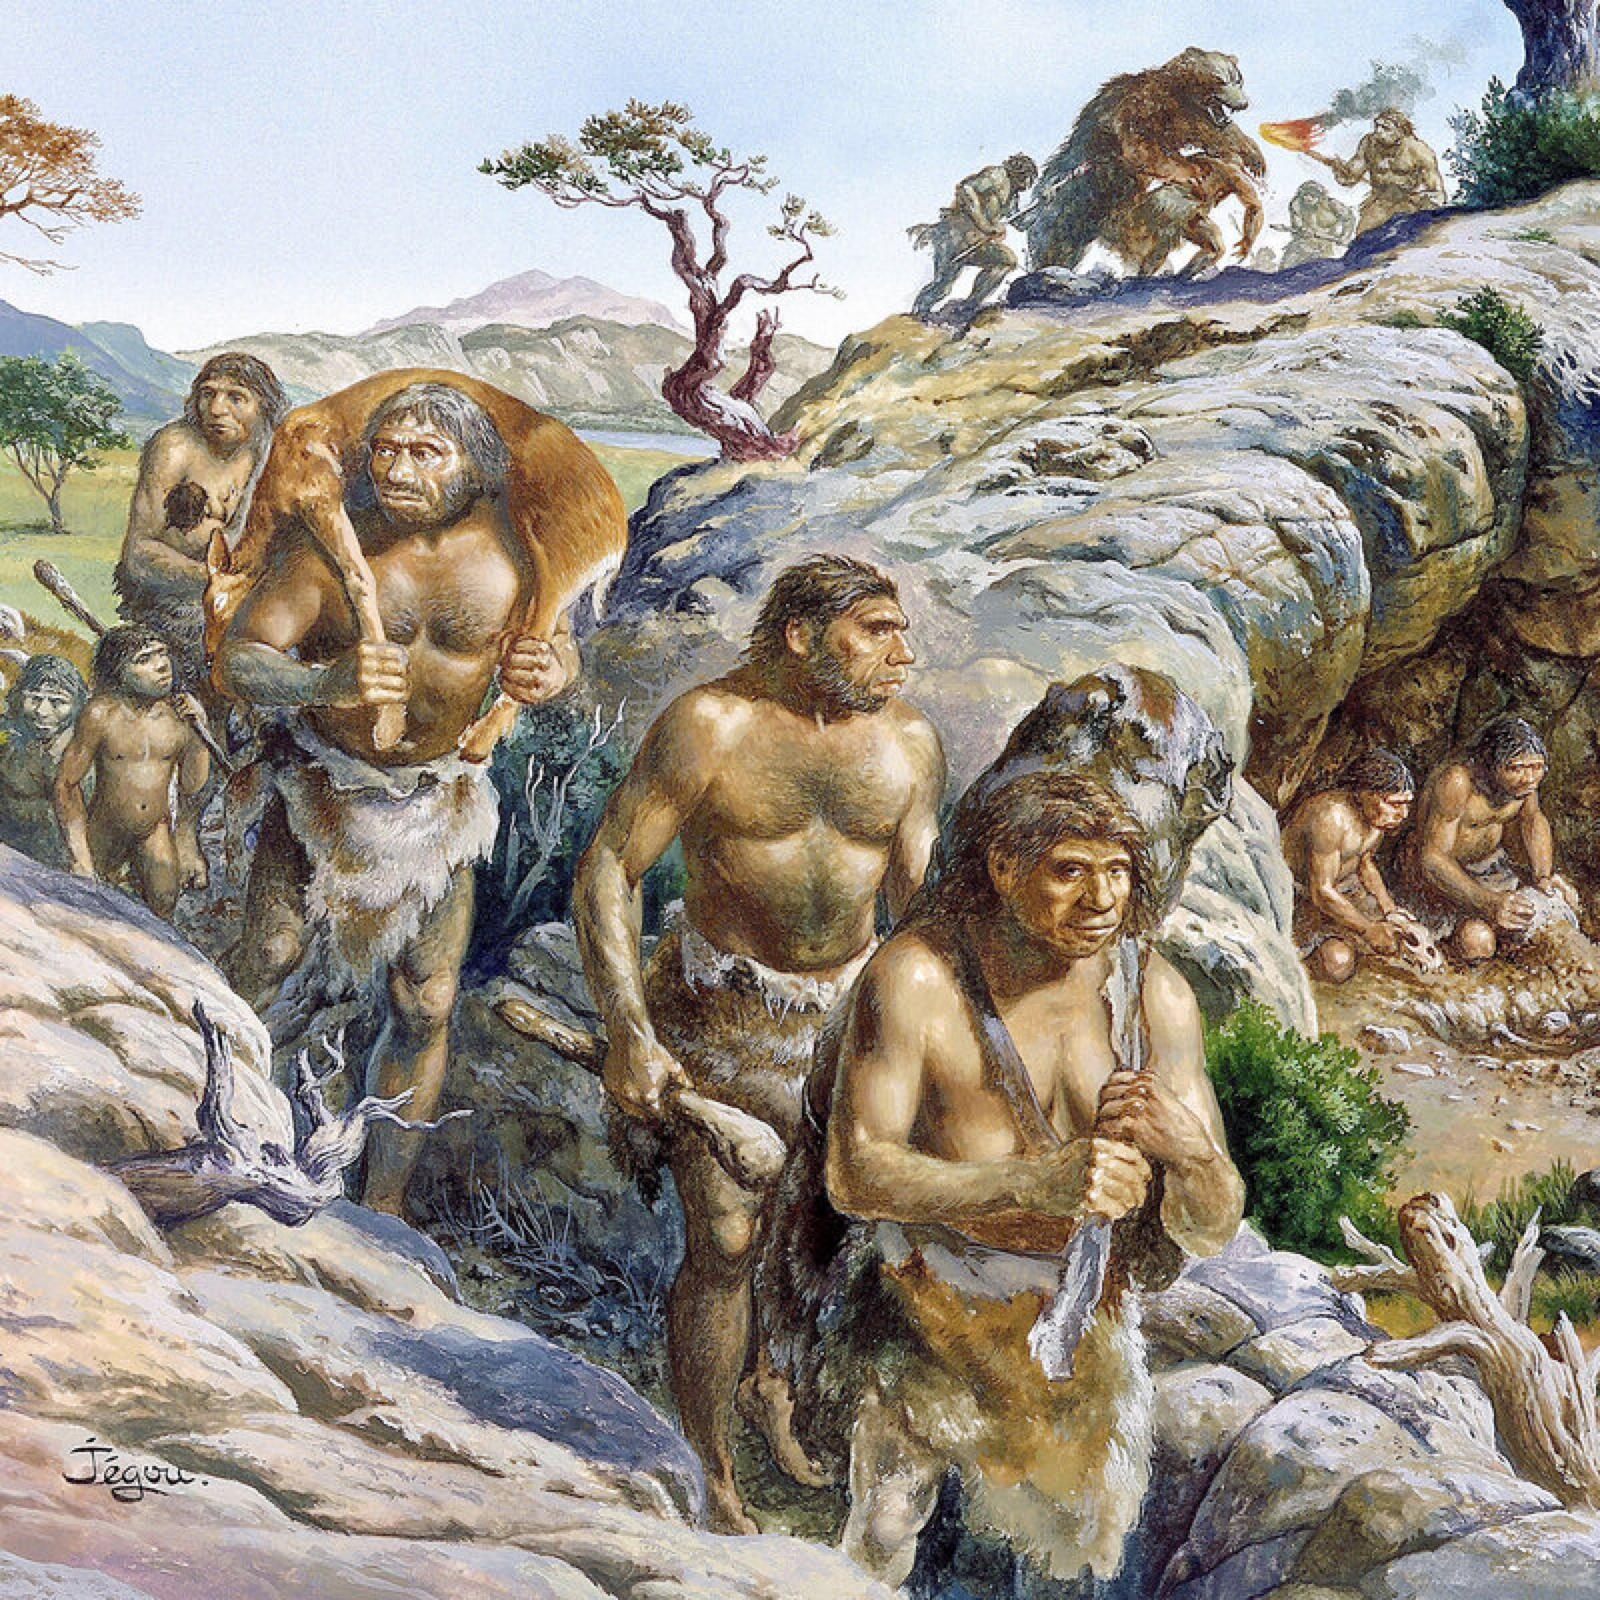
\includegraphics[scale=0.18]{neanderthals}


 \column{0.55\textwidth}
 \begin{itemize}
\item
Neanderthals were a species close to ours (Sapiens, Sapiens). They dominated Europe for almost 0.5 Myr, had brains as large as ours, and dominated lithic technology. However, they never went any further. 
\item It is not clear why Neanderthals went extinct, but presumably it could have been the other way around. In that would have been the case, perhaps a technological civilisation would have never evolved. 
\end{itemize}


\end{columns}
\end{frame}

%\begin{frame}
%\frametitle{Revisiting Drake's equation: ``Best case''}
%%
%%
%%\begin{columns}
%%\column{0.45\textwidth}
%$$
%N = R \times f_{GHZ} \times f_p \times n_e \times f_l \times f_{cl} \times f_i   \times f_c \times L =  10^{-2} \times L 
%$$
% %\column{0.55\textwidth}
% \begin{itemize}
%\item $R  \times f_{GHZ} \times f_p \sim 1 \times 10^{-1} \times 10^{-1} \sim 10^{-2}$
%\item $n_e \sim 1$ (At least one planet is inhabitable in the Solar System)
%\item $f_l \sim 1$ (Life is common).
%\item $f_{cl}\sim  1$ (Once life appears, complex life appears too, sooner or later.)
%\item $f_i \sim 1$ (Once complex life appears, intelligence is inevitable)
%\item $f_{c}\sim  1$ (Once intelligence appears, technological civilisations are inevitable.). 
% 
%\end{itemize}
%%\end{columns}
%\end{frame}


\begin{frame}
\frametitle{Revisiting Drake's equation: the ``pessimist'' hypothesis}
%
%
%\begin{columns}
%\column{0.45\textwidth}
$$
N = R \times f_{GHZ} \times f_p \times n_e \times f_l \times f_{cl} \times f_i   \times f_c \times L = 1 \times 10^{-1} \times 10^{-5} \times10^{-5}  \times 1 L \sim  10^{-11} L
$$
 %\column{0.55\textwidth}
 \begin{itemize}
\item $R  \times f_{GHZ}  \sim 10^{-1}$
\item $f_p \times n_e \times f_l \times f_{cl} \sim 10^{-5} $ (REH, Rare Complex life)
\item $f_i \sim 10^{-5}$ (Mayr's view, Rare's intelligence).
\item $f_{c}\sim  1$ (our species, extinction taken into account in $f_i$). 
\end{itemize}
%\end{columns}

\begin{block}{}

Thus, even if $L$ is as long as the age of the Galaxy ($10^{10}$yr), $N < \sim 1$ (us)
\end{block}

\end{frame}

%\begin{frame}
%\frametitle{Drake's equation in perspective}
%%
%%
%\begin{columns}
%\column{0.45\textwidth}
%\includegraphics[scale=0.25]{drake2}
% \column{0.55\textwidth}
% \begin{itemize}
%\item From ``best'' to ``worst'' case scenario, ``predictions'' differ in 12 orders of magnitude. 
%\item This is without counting $L$ which could be taken between $10^3-10^9$ yr. 
%\item Thus, one extreme case would predict $R = 10^7$ ETCs in the Galaxy
%\item While the other would predict  $R = 10^{-11}$ ETCs in the Galaxy. 
%\item This illustrates the non-predictive nature of Drake's equation, which was always intended as a way to formulate the problem, e.g, the uncertainties.  
%\end{itemize}
%\end{columns}
%\end{frame}

\begin{frame}
\frametitle{Classification of FP solutions}

\begin{itemize}
\item Proposed by Cirkovic in 2009\footnote{Serb. Astron. J.  178 (2009), 1 - 20}.
\end{itemize}

\includegraphics[scale=0.75]{FPclassification.pdf}

\end{frame}

%\begin{frame}
%\frametitle{Solipsist Soluitions}
%
%Solipsist solutions propose that extraterrestrials are or have been present in our vicinity, but have so far been undetected. 
%%The reasons for such non detectability are varied and span a large family of hypothesis. Among them:
%
%\begin{enumerate}
%\item {\bf UFO's} have been observed and are of extraterestial origin. 
%\item {\bf The Zoo hypothesis} of Ball (1973) and the related {\bf Interdict hypothesis} of Fogg (1987), suggest that there is a uniform cultural policy of advanced extraterrestrial civilizations to avoid any form of contact (including having a visible manifestations) with the newcomers to the ``Galactic Club''.
%\item {\bf Directed panspermia} of Crick and Orgel (1973) suggests that Earth has indeed been visited in a distant past with very obvious consequences ---namely the existence of life on Earth! 
%\item {\bf The Planetarium hypothesis} of Baxter (2000) suggests that our astronomical observations do not represent reality, but a form of illusion, created by an advanced technological civilization capable of manipulating matter and energy on interstellar or Galactic scales.
%\item {\bf The Simulation hypothesis} of Bostrom (2003), suggest that we live in a computer simulation of an advanced technological civilization inhabiting the ``real'' universe.
%\end{enumerate}
%
%\end{frame}

\begin{frame}
\frametitle{Catastrophist solutions: Natural hazards}

\begin{columns}
\column{0.45\textwidth}
\includegraphics[scale=0.25]{tauceti}

\column{0.55\textwidth}
\begin{itemize}
\item The risk of cometary/asteroidal bombardment supervolcanism
nearby supernovae etc. might be in general much
higher than we infer from the recent history of
Earth. These natural hazards can break the evolutionary chain leading
to the emergence of intelligent observers.
\item An interesting example is the Sun-like Tau Ceti, which contains four rocky planets (Super-Earths), two of which are in the habitable zone. But in addition, the system contains 
 a massive debris disk, analogous to the Kuiper belt but with 10 times more material. Presumably, then, the planets in Tau Ceti are subjected to much more severe impact
stress than Earth has been during the course
of its geological and biological history.
\end{itemize}
\end{columns}

\end{frame}

%\begin{frame}
%\frametitle{Catastrophist solutions: Dark Forest/Berserker hypothesis}
%
%\begin{columns}
%\column{0.45\textwidth}
%\includegraphics[scale=0.16]{berserkers}
%
%\column{0.55\textwidth}
%\begin{itemize}
%
%\item A particularly nasty  version of Tipler's scenario posits that self-replicating von Neumann probes are
%not peaceful explorers  but intentionally or accidentally
%created destructive weapons. This leads to  a very hostile ecological system
%Depending on the
%unknown mode of operation of the berserker, they might be homing on
%the sources of coherent radio emission (indi-
%cating a young civilization to be eliminated) or
%might be automatically sweeping the Galaxy
%in search for such adversaries. 
%
%\item This disturbing hypothesis is, BTW, consistent with Brin (1983)
%with (no) observation and non-exclusivity. 
%\end{itemize}
%\end{columns}
%
%\end{frame}
%
\begin{frame}
\frametitle{Towards a Hard (physical) solution}

\begin{itemize}

\item 
An astrophysical (necessarily ``hard'') explanation of FP would be  preferable over a sociological one, and presumably more testable and less speculative than
many of the REH propositions.

\item  Much of the tension caused by Fermi’s paradox stems from the tacit
assumption of equilibrium state. Instead, James Annis\footnote{Annis, J.: 1999a, J. Brit. Interplanet. Soc., 52, 19.}  has proposed the phase transition
idea, which is a prototype disequilibrium hypothesis.

\item A plausible astrophysical scenario
for a delay in the emergence of intelligent observers and their technological civilizations
is the existence in the Galaxy of a global regulation
mechanism. Such a mechanism could occasionally reset astrobiological ``clocks'' all
over the GHZ and in a sense re-synchronize them. Thus:
\end{itemize}
 
\begin{block}{}

There is no Fermi's
paradox, since the relevant timescale is the
time elapsed since the last ``reset'' of astrobiological clocks and this can be substantially
smaller than the age of the Milky Way or
$t_M - t_E.$

\end{block}

\end{frame}

\begin{frame}
\frametitle{Global regulation by mean of GRB's}

%phasetransition
\begin{columns}
\column{0.45\textwidth}
\includegraphics[scale=0.46]{extinction}

Galactic Habitable Zone in 1-D simple quantitative model. Presented is the number of planets that
have achieved noogenesis at least once (cumulative plot), as a function of the age of the Milky Way thin disk
stellar population and the mean extinction probability Q per global catastrophe
\column{0.55\textwidth}
\begin{itemize}

\item Any form of catastrophic event affecting planetary biospheres
in the Milky Way Galaxy will reduce the hypothetical civilizations’ ages and, thus, reduce
the tension inherent in Fermi’s paradox. Moreover, global catastrophic events affecting
large parts of GHZ will tend to reset local astrobiological clocks nearly
simultaneously, thus significantly decreasing the probability of existence of extremely old
civilizations.

\item Global regulation has been assumed to occur in form of GRBs, modelled as random
events occurring with exponentially decreasing frequency
\end{itemize}
$$ v(t) = v_0 \exp{-\frac{t}{t_\gamma}}\, \, (t_\gamma  \sim 5 Gyr)$$


\end{columns}

\end{frame}

\begin{frame}
\frametitle{ Phase Transition}

%phasetransition
\begin{columns}
\column{0.45\textwidth}
\includegraphics[scale=0.46]{phasetransition}

Schematically illustrated,
evolution of astrobiological complexity
in the history of the Milky
Way according to the phase transition
hypothesis
\column{0.55\textwidth}
\begin{itemize}

\item  At very early epochs (I), the Galaxy was completely dead;  For most of the Galaxy history its astrobiological
structure was in a state we denote with “II”—containing enclaves and pockets of simple life,
but the emergence of complex life-forms and of intelligent was strongly suppressed by global regulation mechanisms. 

\item However, the frequency of resetting events decreased due to the astrophysical evolution of the
Galaxy (e.g, decrease of GRBs), and at some time  the balance shifts toward
high probability of complex intelligent observers emerging and creating large interstellar
civilizations. That is the epoch of phase transition. 

\end{itemize}

\end{columns}

\end{frame}

\begin{frame}
\frametitle{ The Astrobiological Phase Transition  model }

\begin{enumerate}

\item  We are currently living in a disequilibrium period of the phase
transition. $\sim 10^8$ years ago our Galaxy was dead as far as high-complexity life was
concerned; $\sim 10^8$ years from now the Galaxy will be entirely filled with high-complexity life.
\item The phase transition is governed by an intricate interplay between (a) the natural
tendency of life to grow, spread, complexify, and fill all available ecological niches,
and (b) global regulations mechanism(s).
\item GRBs are the best candidates for such a global regulation mechanism.
\item The APT avoids the Fermi Paradox.
\end{enumerate}

\end{frame}

\begin{frame}
\frametitle{ The ATP Model Predictions }

\begin{enumerate}

\item  We shall not find any traces or remnants of intelligent societies much older than ours
anywhere in the Galaxy.
\item We shall not receive and perceive any extragalactic CETI signals, nor shall we detect
activities of advanced extragalactic societies, at least not before humans are on the way
of becoming (or joining) the Kardashev Type III super-society. This is the consequence
of roughly parallel secular evolution of the global regulation mechanisms in the Milky
Way and other nearby similar spiral galaxies.
\item The ages of discovered societies will be comparable to our own, i.e. incompatible with
any broad distribution (uniform, broad Gaussian, etc.).
\item We shall find ubiquitous traces of low-complexity life, from other habitats in our Solar
System (Mars, Europa) to the other planetary systems, unbound planets and even possibly
ISM and proto-stellar clouds. This is in agreement with Ward and Brownlee’s the “Rare
Earth” hypothesis. 
\item We will find 
evidence of high-energy $\gamma$ and cosmic-ray bombardment episodes approximately
coincident with some of the major known Earth-biosphere extinction events.
\end{enumerate}

\end{frame}

\begin{frame}

\frametitle{ The Advanced Civilization is US}

\begin{enumerate}

\item  There are no super-advanced civilizations in the Galaxy, as there are no Gods in Mount Olympus. {\bf For all practical purposes, we are alone}.
\item Is up to us to become an advanced civilisation, instead of a extinct one. {\bf No one is gonna save us from ourselves.}.
\item Copernicanism still apply. We are typical and at the same time, {\bf we are unique}.
\end{enumerate}
\end{frame}


\end{document}